\documentclass[11pt,a4paper]{article}
\usepackage[utf8]{inputenc}
\usepackage[T1]{fontenc}
\usepackage{geometry}\geometry{margin=2.5cm}
\usepackage{graphicx,amsmath,amssymb,booktabs,longtable,listings,xcolor,hyperref,float,enumitem,fancyhdr,tikz}
\usetikzlibrary{shapes.geometric,arrows.meta,positioning}

\definecolor{codebg}{RGB}{245,245,245}
\definecolor{codeframe}{RGB}{200,200,200}
\lstset{language=Python,basicstyle=\ttfamily\footnotesize,backgroundcolor=\color{codebg},frame=single,rulecolor=\color{codeframe},breaklines=true,numbers=left,numberstyle=\tiny\color{gray},keywordstyle=\color{blue},commentstyle=\color{green!50!black},stringstyle=\color{red!70!black},showstringspaces=false}

\pagestyle{fancy}\fancyhf{}
\lhead{LINE-2D Shape-Based Matching}\rhead{Technical Document}\cfoot{\thepage}

\title{\textbf{LINE-2D Shape-Based Matching}\\[4pt]\large Technical Handover Document\\[2pt]\normalsize Wafer Alignment System -- QES (Asia-Pacific) Sdn Bhd}
\author{Engineering Team}\date{May 2026}

\begin{document}
\maketitle\tableofcontents\newpage

% ============================================================
\section{Executive Summary}
This document describes the LINE-2D shape-based template matching subsystem used in the Wafer Alignment application. The algorithm locates a trained template pattern in a search image by comparing quantised gradient orientations. It is a Python port of the C++ SBM\_line2D implementation (reference: \texttt{SeanYan604/SBM\_line2D}).

Key capabilities: rotation-invariant matching ($0$--$360\degree$, configurable step), multi-scale support, sub-pixel position and angle refinement, and coarse-to-fine pyramid acceleration for high-resolution ($>2000$\,px) images.

% ============================================================
\section{Architecture Overview}

\subsection{MVVM Layer Mapping}
\begin{center}
\begin{tabular}{lll}\toprule
\textbf{Layer} & \textbf{File} & \textbf{Role}\\\midrule
Service & \texttt{linemod\_matcher.py} & Core algorithm (1330 lines)\\
ViewModel & \texttt{pattern\_viewmodel.py} & UI logic, config, caching\\
View & \texttt{pattern\_tab.py} & Tkinter widgets\\
Model & \texttt{recipe\_model.py} & XML recipe persistence\\
Model & \texttt{app\_state.py} & Shared mutable state\\
Integration & \texttt{zmq\_server.py} & ZeroMQ TCP interface\\\bottomrule
\end{tabular}
\end{center}

\subsection{Dependency Graph}
\begin{center}
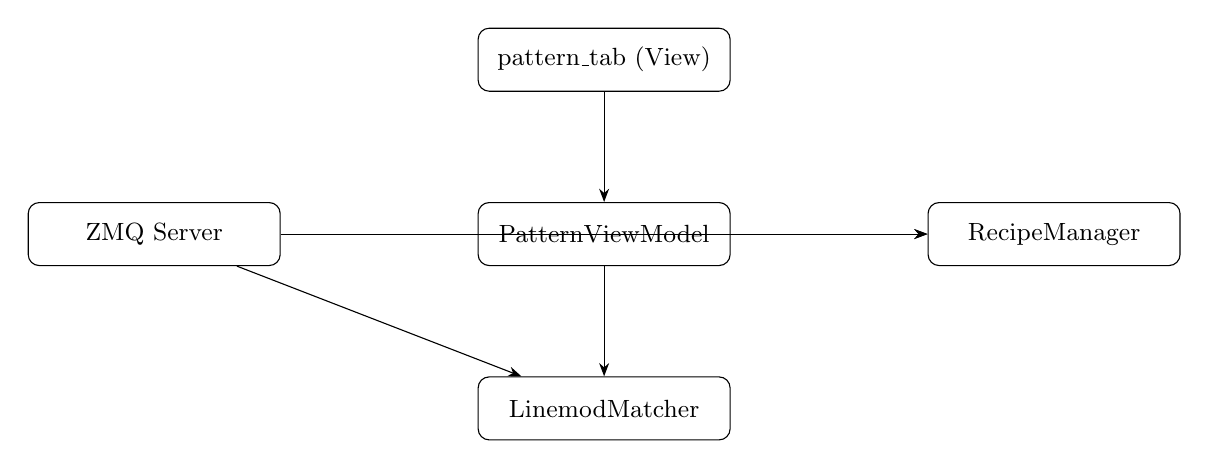
\begin{tikzpicture}[node distance=1.4cm,every node/.style={draw,rounded corners,minimum width=3.2cm,minimum height=0.8cm,font=\small}]
\node(V){pattern\_tab (View)};
\node(VM)[below=of V]{PatternViewModel};
\node(S)[below=of VM]{LinemodMatcher};
\node(R)[right=2.5cm of VM]{RecipeManager};
\node(Z)[left=2.5cm of VM]{ZMQ Server};
\draw[-{Stealth}](V)--(VM);
\draw[-{Stealth}](VM)--(S);
\draw[-{Stealth}](VM)--(R);
\draw[-{Stealth}](Z)--(S);
\draw[-{Stealth}](Z)--(R);
\end{tikzpicture}
\end{center}

% ============================================================
\section{Algorithm Pipeline}

The matching pipeline has two phases: \textbf{offline} (template generation) and \textbf{online} (search-image matching).

\subsection{Phase 1 -- Template Generation (\texttt{generate\_templates})}
\begin{enumerate}
\item \textbf{Rotation \& Scale Grid}: For each $(angle, scale)$ pair the base template image is rotated and scaled via \texttt{cv2.warpAffine}. Default: $5\degree$ step $\times$ 1 scale $= 72$ templates.
\item \textbf{Mask Handling}: A rotation mask (all-white image transformed identically) prevents border artefacts. An optional user-drawn detection mask restricts feature extraction.
\item \textbf{Pyramid Construction}: For each pyramid level $l \in \{0,1,2\}$, the image is downsampled by $2^l$ via \texttt{cv2.pyrDown}.
\item \textbf{Gradient Quantisation}: At each level, Sobel gradients $\rightarrow$ angle $\rightarrow$ 8 orientation bins (see \S\ref{sec:quantize}).
\item \textbf{Feature Extraction}: $N$ spatially-scattered features selected by gradient magnitude (see \S\ref{sec:features}).
\item \textbf{Bounding-Box Crop}: \texttt{\_crop\_templates} computes the tightest bounding box and makes feature coordinates relative.
\item \textbf{NumPy Pre-caching}: Feature $(x,y,label)$ arrays cached as \texttt{int32} vectors for inner-loop speed.
\end{enumerate}

Template generation is parallelised with \texttt{ThreadPoolExecutor} (up to 8 workers). OpenCV/NumPy release the GIL so threads run in parallel.

\subsection{Phase 2 -- Online Matching (\texttt{match})}
Two execution paths exist, selected automatically by image size:
\begin{itemize}
\item \textbf{Single-Level} ($\leq 2000$\,px): Full-resolution scan.
\item \textbf{Pyramid} ($> 2000$\,px): Coarse-to-fine (see \S\ref{sec:pyramid}).
\end{itemize}

% ============================================================
\section{Core Algorithms}

\subsection{Gradient Quantisation}\label{sec:quantize}
\textbf{Function}: \texttt{\_quantize\_gradients(src, weak\_threshold, fast\_mode, kernel\_size)}

\begin{enumerate}
\item Convert to float32 grayscale.
\item Optional Gaussian blur (auto-sigma for images $>1500$\,px, or explicit kernel).
\item Sobel derivatives: $dx = \text{Sobel}(I, x)$, $dy = \text{Sobel}(I, y)$, $ksize=3$.
\item Magnitude: $M = \sqrt{dx^2 + dy^2}$; Angle: $\theta = \text{atan2}(dy, dx) \bmod 360\degree$.
\item Quantise to 16 bins then fold to 8: \texttt{quant\_8 = (angle * 16/360).astype(uint8) \& 7}.
\item \textbf{Adaptive threshold}: If \texttt{weak\_threshold < 0}, use the $|\text{value}|$-th percentile of non-zero magnitudes.
\end{enumerate}

\paragraph{Hysteresis Mode (fast\_mode=False)}
For each of 8 orientation bins, count votes in a $ks \times ks$ neighbourhood via \texttt{cv2.filter2D}. Accept a pixel only if $M > \text{threshold}$ \textbf{and} the winning bin has $\geq \lceil ks^2/2 \rceil + 1$ votes. Kernel size: auto $= \min(\max(3, \lfloor 3 \cdot \text{maxdim}/1500 \rfloor) | 1, 9)$.

\paragraph{Fast Mode (fast\_mode=True)}
Skip hysteresis; accept any pixel where $M > \text{threshold}$. Used for search images where speed matters.

\paragraph{Output} A \texttt{uint8} image where each pixel is a power-of-2 bit ($2^{\text{bin}}$) or 0.

\subsection{Orientation Spreading}\label{sec:spread}
\textbf{Function}: \texttt{\_spread(quantized, T)}

OR-dilates each of the 8 bit-planes independently with a $(2T{-}1) \times (2T{-}1)$ rectangular kernel via \texttt{cv2.dilate}, then ORs the results. This creates tolerance to small spatial misalignment.

Default $T$ values per pyramid level: $[4, 8, 16]$.

\subsection{Response Map LUTs}\label{sec:lut}
\textbf{Function}: \texttt{\_build\_response\_luts()} $\rightarrow$ 8 tables of 256 entries.

For each template label $L \in \{0..7\}$ and each possible spread byte $v \in \{0..255\}$:
\[
\text{LUT}[L][v] = \begin{cases}4 & \text{if bit } L \text{ is set in } v\\1 & \text{if a neighbour bit } (L\pm 1 \bmod 8) \text{ is set}\\0 & \text{otherwise}\end{cases}
\]

Response maps are computed via \texttt{cv2.LUT(spread\_img, LUT[label])} -- a single vectorised lookup per label.

\subsection{Scattered Feature Selection}\label{sec:features}
\textbf{Function}: \texttt{\_extract\_scattered\_features(quantized, magnitude, N, mask)}

\begin{enumerate}
\item Collect all non-zero quantised pixels (optionally masked).
\item Sort by descending gradient magnitude.
\item Greedily select $N$ features with minimum-distance constraint. Distance starts at $d = \text{perimeter} / (0.8N)$ and shrinks by $15\%$ per pass.
\item Uses spatial grid hashing: distance checks are $O(9 \times k)$ per candidate instead of $O(n)$.
\end{enumerate}

\subsection{Score Map Computation}
For each template, accumulate response values at feature locations:
\[
S(r,c) = \sum_{i=1}^{N_\text{feat}} \text{ResponseMap}[\text{label}_i][r + y_i,\; c + x_i]
\]
Similarity: $\text{sim}(r,c) = 100 \times S(r,c) \;/\; (4 \times N_\text{valid})$.

Features are sorted by label to improve L2 cache hit rate (same response map accessed consecutively).

Score maps use \texttt{int16} dtype (max $128 \times 4 = 512 < 32767$).

\subsection{Sub-Pixel Position Refinement}
\textbf{Function}: \texttt{\_subpixel\_refine(score\_map, r, c)}

3-point parabolic fit on each axis independently:
\[
\delta_x = \frac{S(r,c{-}1) - S(r,c{+}1)}{2\bigl(S(r,c{-}1) - 2S(r,c) + S(r,c{+}1)\bigr)}, \quad \text{clamped to } [-0.5, +0.5]
\]

\subsection{Angular Sub-Pixel Interpolation}
\textbf{Function}: \texttt{\_angular\_interpolate(matches)}

Given the best discrete match at angle $\theta_0$ with score $S_0$, and scores $S_{-}$, $S_{+}$ from the adjacent angle templates:
\[
\delta_\theta = \frac{\Delta\theta}{2} \cdot \frac{S_{-} - S_{+}}{S_{-} - 2S_0 + S_{+}}, \quad |\delta_\theta| \leq \frac{\Delta\theta}{2}
\]

\subsection{Non-Maximum Suppression}
\textbf{Function}: \texttt{\_nms(matches)}

Sort by score descending. Keep a match only if its Euclidean distance to all previously kept matches exceeds \texttt{NMS\_DISTANCE} (default 30\,px).

% ============================================================
\section{Pyramid Matching}\label{sec:pyramid}
\textbf{Function}: \texttt{\_match\_pyramid(search\_gray, threshold)}

\subsection{Coarse Pass (Level $N$)}
\begin{enumerate}
\item Downsample search image by $2^N$ via \texttt{cv2.pyrDown}. Level $N = \min(\text{PYRAMID\_LEVELS}-1, \lceil\log_2(\text{maxdim}/1200)\rceil)$.
\item Quantise, spread (with $T_N$), compute response maps at coarse resolution.
\item Score each template using only the first \texttt{COARSE\_NUM\_FEATURES} (default 32) features.
\item Lower threshold: $\max(0.3 \times \text{threshold}, 15)$.
\item Keep top candidate per template. Cap total to \texttt{MAX\_FINE\_CANDIDATES}.
\end{enumerate}

\subsection{Fine Pass (Level 0)}
\begin{enumerate}
\item Cluster overlapping ROI windows into \emph{super-ROIs}.
\item For each super-ROI: quantise (fast mode), spread, build response maps \emph{once}.
\item Score each candidate template within its sub-window of the super-ROI.
\item Full feature set ($N=128$) at full resolution for precise localisation.
\end{enumerate}

% ============================================================
\section{Configuration Reference}

\begin{longtable}{p{4.2cm}p{2cm}p{7.5cm}}\toprule
\textbf{Parameter} & \textbf{Default} & \textbf{Description}\\\midrule\endhead
\texttt{ANGLE\_STEP} & 5 & Degrees between rotation templates\\
\texttt{SCALE\_MIN/MAX} & 1.0/1.0 & Scale range (0.8--1.2 for Full Search)\\
\texttt{SCALE\_STEP} & 0.1 & Scale increment\\
\texttt{WEAK\_THRESHOLD} & $-70$ & Gradient threshold. Negative = percentile-adaptive\\
\texttt{NUM\_FEATURES} & 128 & Features per template level\\
\texttt{HYSTERESIS\_KERNEL} & 0 & Majority-vote kernel size (0=auto)\\
\texttt{T\_PYRAMID} & [4,8,16] & Spread $T$ per pyramid level\\
\texttt{MATCH\_THRESHOLD} & 50.0 & Minimum similarity (0--100)\\
\texttt{NMS\_DISTANCE} & 30 & Non-max suppression radius (px)\\
\texttt{FAST\_SEARCH\_QUANTIZE} & True & Skip hysteresis on search images\\
\texttt{COARSE\_NUM\_FEATURES} & 32 & Features for coarse pass\\
\texttt{MAX\_COARSE\_CANDIDATES} & 2 & Top candidates per template (coarse)\\
\texttt{MAX\_FINE\_CANDIDATES} & 5 & Cap before fine pass\\\bottomrule
\end{longtable}

% ============================================================
\section{Search Modes (UI)}

\begin{tabular}{llll}\toprule
\textbf{Mode} & \textbf{ANGLE\_STEP} & \textbf{Scale} & \textbf{Templates}\\\midrule
Simple (Fast) & 360 (=only 0\textdegree) & 1.0 & 1\\
With Rotation & 10 & 1.0 & 36\\
Full Search & 10 & 0.8--1.2 & $\sim$180\\\bottomrule
\end{tabular}

% ============================================================
\section{Data Structures}

\subsection{Feature}
\begin{lstlisting}
class Feature:
    __slots__ = ['x', 'y', 'label']  # x,y: position; label: orientation bin 0-7
\end{lstlisting}

\subsection{TemplatePyr}
\begin{lstlisting}
class TemplatePyr:
    __slots__ = ['width', 'height', 'tl_x', 'tl_y',
                 'pyramid_level', 'features',
                 'feat_xs_arr', 'feat_ys_arr', 'feat_labels_arr']
\end{lstlisting}

\subsection{Template Pyramid Entry (dict)}
\begin{lstlisting}
{ 'angle': float, 'scale': float,
  'templates': [TemplatePyr, ...],  # one per pyramid level
  'size': (width, height) }
\end{lstlisting}

\subsection{Match Result (dict)}
\begin{lstlisting}
{ 'x': float, 'y': float,          # sub-pixel centre
  'angle': float,                   # refined angle (degrees)
  'angle_discrete': float,          # original grid angle
  'angle_interp_delta': float,      # interpolation offset
  'scale': float, 'score': float,   # 0-100 similarity
  'template_id': int,
  'bbox': (x, y, w, h) }
\end{lstlisting}

% ============================================================
\section{ZMQ Integration}

\subsection{PM\_REQ Command}
\begin{verbatim}
PM_REQ "<image_path>" "<recipe_path>"
\end{verbatim}
Response (JSON): \texttt{\{"status":"ok", "x":..., "y":..., "angle":..., "score":..., "delta\_x":..., "delta\_y":...\}}

\subsection{TEACH\_REQ Command}
\begin{verbatim}
TEACH_REQ "<image_path>" "<recipe_path>"
\end{verbatim}
Opens interactive OpenCV ROI selector. Operator crops template, optionally draws detection mask. Saves to recipe XML.

% ============================================================
\section{Recipe XML Schema (FindPattern)}
\begin{lstlisting}[language=XML]
<FindPattern>
  <MatchThreshold>50.0</MatchThreshold>
  <NumFeatures>128</NumFeatures>
  <GradThrPct>70.0</GradThrPct>
  <TSpread>4</TSpread>
  <HystKernel>0</HystKernel>
  <SearchMode>Simple (Fast)</SearchMode>
  <TemplatePath>C:\...\template.png</TemplatePath>
  <TemplateCropCX>512.0</TemplateCropCX>
  <TemplateCropCY>310.0</TemplateCropCY>
  <DetectionMaskPath></DetectionMaskPath>
</FindPattern>
\end{lstlisting}

% ============================================================
\section{Performance Characteristics}

\begin{tabular}{lrrr}\toprule
\textbf{Phase} & \textbf{919px} & \textbf{2560px} & \textbf{5120px}\\\midrule
Quantise (fast) & 5\,ms & 15\,ms & 50\,ms\\
Spread ($T{=}4$) & 8\,ms & 25\,ms & 90\,ms\\
Response Maps & 3\,ms & 10\,ms & 35\,ms\\
Scoring (1 tmpl) & 10\,ms & 80\,ms & 300\,ms\\
Scoring (72 tmpl) & 200\,ms & -- & --\\
Pyramid total & -- & 180\,ms & 400\,ms\\\bottomrule
\end{tabular}

Memory: Response maps use \texttt{int16} (halves bandwidth vs \texttt{int32}). Rotated template images are \emph{not} stored; regenerated on-demand for visualisation.

% ============================================================
\section{Detection Mask System}

Users can draw a polygon mask on the template to exclude regions (e.g.\ wafer boundary curvature). Implementation:
\begin{enumerate}
\item \texttt{mask\_editor.py}: OpenCV interactive polygon drawing window with auto-detection of wafer boundary.
\item Mask stored as \texttt{<template>\_mask.png} alongside the template.
\item Passed to \texttt{\_extract\_scattered\_features} as a binary mask: features only extracted where $\text{mask} > 0$.
\item Mask is rotated/scaled identically to the template during \texttt{generate\_templates}.
\end{enumerate}

% ============================================================
\section{Smart Template Caching}

The \texttt{PatternViewModel} tracks a config fingerprint string:
\begin{lstlisting}
f"{NUM_FEATURES}_{WEAK_THRESHOLD}_{T_PYRAMID}_{HYSTERESIS_KERNEL}_{ANGLE_STEP}_{SCALE_MIN}_{SCALE_MAX}_{img_hash}_{mask_hash}"
\end{lstlisting}
Templates are only regenerated when this string changes. This avoids redundant $\sim$2\,s rebuilds during slider tuning.

% ============================================================
\section{Known Limitations \& Future Work}
\begin{itemize}
\item No GPU acceleration (CUDA Sobel/dilate was prototyped but PCIe overhead exceeded gains for template-sized crops).
\item Scale search is coarse ($0.1$ step); finer steps increase template count linearly.
\item Single-level fallback (\texttt{\_match\_single\_level}) is slow for images $>2000$\,px; pyramid path should always be preferred.
\item No rotation-invariant NMS (matches at different angles near the same position may both survive).
\end{itemize}

% ============================================================
\section{File Reference}
\begin{longtable}{p{5.5cm}p{8cm}}\toprule
\textbf{File} & \textbf{Purpose}\\\midrule
\texttt{app/services/linemod\_matcher.py} & Core LINE-2D algorithm (1330 lines)\\
\texttt{app/viewmodels/pattern\_viewmodel.py} & UI business logic, config application, timing chart\\
\texttt{app/views/pattern\_tab.py} & Tkinter tab UI (sliders, buttons, image display)\\
\texttt{app/views/mask\_editor.py} & Interactive polygon mask editor\\
\texttt{app/models/recipe\_model.py} & XML recipe read/write\\
\texttt{app/models/app\_state.py} & Shared state (template crop centre, mask, flags)\\
\texttt{app/services/zmq\_server.py} & ZMQ server (PM\_REQ, TEACH\_REQ handlers)\\\bottomrule
\end{longtable}

\end{document}
